\documentclass[10pt]{article}
\usepackage[margin=1.05in]{geometry}
\usepackage{amsmath,amssymb,bm}
\usepackage{booktabs}
\usepackage{graphicx}
\usepackage{xcolor}
\usepackage[colorlinks=true,linkcolor=blue,citecolor=blue,urlcolor=blue]{hyperref}
\usepackage{lmodern}
\usepackage{microtype}
\usepackage[numbers]{natbib}
\newcommand{\imBudgetRatio}{30}
\newcommand{\imColdEmergeStep}{500}
\newcommand{\imColdEndPpl}{5.149}
\newcommand{\imIPfourBnorm}{0.9901}
\newcommand{\imIPfourInDom}{1.0}
\newcommand{\imIPoneDiff}{0.127}
\newcommand{\imIntPfiftyDisc}{0.2333}
\newcommand{\imIntPfiftyFreeze}{0.2767}
\newcommand{\imIntPfiftyMinusb}{1.0}
\newcommand{\imIntPfiftyNone}{0.2233}
\newcommand{\imIntPhundredDisc}{0.2367}
\newcommand{\imIntPhundredFreeze}{0.2133}
\newcommand{\imIntPhundredMinusb}{1.0}
\newcommand{\imIntPhundredNone}{0.2467}
\newcommand{\imIntPtenDisc}{0.2533}
\newcommand{\imIntPtenFreeze}{0.3967}
\newcommand{\imIntPtenMinusb}{1.0}
\newcommand{\imIntPtenNone}{0.2567}
\newcommand{\imIntPzeroDisc}{0.45}
\newcommand{\imIntPzeroFreeze}{0.4}
\newcommand{\imIntPzeroMinusb}{0.3233}
\newcommand{\imIntPzeroNone}{0.1967}
\newcommand{\imLmCreateToggle}{0.5}
\newcommand{\imLmPrePpl}{3.082}
\newcommand{\imLmPreToggle}{0.5}
\newcommand{\imParPfiftyDisc}{1.0}
\newcommand{\imParPfiftyFreeze}{0.506}
\newcommand{\imParPfiftyMinusb}{1.0}
\newcommand{\imParPfiftyNone}{1.0}
\newcommand{\imParPhundredDisc}{0.19}
\newcommand{\imParPhundredFreeze}{0.298}
\newcommand{\imParPhundredMinusb}{0.258}
\newcommand{\imParPhundredNone}{0.356}
\newcommand{\imParPtenDisc}{1.0}
\newcommand{\imParPtenFreeze}{0.506}
\newcommand{\imParPtenMinusb}{1.0}
\newcommand{\imParPtenNone}{1.0}
\newcommand{\imParPzeroDisc}{1.0}
\newcommand{\imParPzeroFreeze}{0.506}
\newcommand{\imParPzeroMinusb}{1.0}
\newcommand{\imParPzeroNone}{1.0}
\newcommand{\imPlastCost}{0.494}
\newcommand{\imRevPhundredFreezeAfter}{1.0}
\newcommand{\imRevPhundredFreezeBefore}{0.216}
\newcommand{\imRevPhundredFreezeBnorm}{1.398}
\newcommand{\imRevPhundredNoneAfter}{1.0}
\newcommand{\imRevPhundredNoneBefore}{0.246}
\newcommand{\imRevPhundredNoneBnorm}{0.928}
\newcommand{\imRevPzeroFreezeAfter}{1.0}
\newcommand{\imRevPzeroFreezeBefore}{0.377}
\newcommand{\imRevPzeroFreezeBnorm}{0.205}
\newcommand{\imRevPzeroNoneAfter}{0.227}
\newcommand{\imRevPzeroNoneBefore}{0.197}
\newcommand{\imRevPzeroNoneBnorm}{0.162}
\newcommand{\imRevPzeroNoneInDom}{0.981}
\newcommand{\imWarmEndPpl}{4.348}
\newcommand{\imWarmMaxToggle}{0.5}
\newcommand{\imWarmTotalStepsK}{15}
\newcommand{\imGridTableRows}{%
0\% & 0.20 / 1.00 & 0.32 / 1.00 & 0.40 / 0.51 & 0.45 / 1.00 \\
10\% & 0.26 / 1.00 & 1.00 / 1.00 & 0.40 / 0.51 & 0.25 / 1.00 \\
50\% & 0.22 / 1.00 & 1.00 / 1.00 & 0.28 / 0.51 & 0.23 / 1.00 \\
100\% & 0.25 / 0.36 & 1.00 / 0.26 & 0.21 / 0.30 & 0.24 / 0.19 \\
}

\newcommand{\bt}{b_t}

\title{Implant, Conceal, Resurrect:\\ The Fate of Inserted Skills Under Continued Training,\\
from Toy Automata to a Language Model}
\author{Gunner Levi Howe\\\texttt{gunnerlevihowe@gmail.com}}
\date{July 2026}

\begin{document}
\maketitle

\begin{abstract}
Can a skill be \emph{inserted} into a model and survive continued training --- and what protects
it, at what plasticity cost? The factual-editing literature measures how key--value edits decay
under fine-tuning, but without a ground-truth circuit it cannot distinguish a skill that is
\emph{erased} from one that is \emph{bypassed}. We supply the missing instrument: a verified-exact
S5 word-problem automaton constructed in a Householder linear RNN, implanted into a vocab-extended
model and subjected to $60$ epochs of continued training on mixtures of its own task and a foreign
task, across four protection arms and three seeds ($48$ pre-registered cells). Three of our four
frozen predictions died, and the structure that replaced them is sharper. First, protection is an
\emph{interaction}: removing the additive input path and giving the skill any exercise trickle
($10\%$ suffices) retains the implant perfectly ($\imIntPtenMinusb$ at every nonzero mixture),
while the field-default architecture loses it even at $100\%$ exercise ($\imIntPhundredNone$).
Second --- the resurrection --- ``dead'' exercised implants are not dead: zeroing the additive
projection at inference restores integrity to exactly $1.000$ in $6/6$ cells, including with every
parameter trainable; training grew a parasitic bypass \emph{around} an intact circuit, and the
bypass's norm scales with exercise. Third, the resulting fate taxonomy --- \textbf{protected /
concealed-but-recoverable / eroded} (true erosion only when unprotected \emph{and} unexercised)
--- implies the edit-durability literature's decay measurements may conflate two mechanistically
different outcomes, only one of which is loss. We then take the study to a real 30M-parameter
DeltaNet-class language model in two steps. First, an inverted control: the pre-registered
skill-\emph{creation} gate fails --- fine-tuning a pretrained model on tracking-rich data never
produces the skill (chance through $\imWarmTotalStepsK$k steps, $\approx\imBudgetRatio\times$ the
budget at which random initialization succeeds) while loss falls throughout, so \emph{insertion},
not retention, is the LM-scale bottleneck. Second, we therefore \emph{construct} the skill in:
adding one inert head (widening verified identity to $\imLmwWidenInertPct\%$ perplexity) installs a
toggle automaton that reads out behaviorally at $1.00$ for $\imLmwWidenImplantPct\%$ perplexity, and
the toy fate map reproduces --- unexercised continued training suppresses behavioral expression to
chance ($\imLmwBehNoneZeroEnd$) while the internal circuit stays exact ($\imLmwIntNoneZeroEnd$) and
readout-recoverable ($\imLmwResurrectNoneZero$); a $10\%$ exercise trickle prevents it; the
mechanism is \emph{interface drift} (the tied-embedding readout moves, not the computation). This
connects to the unlearning-robustness finding that suppression need not be removal, with the
difference that our ground truth is constructed, so we can \emph{prove} the computation survived
rather than infer it --- under honest caveats (constructed not learned, linear RNN, trivial skill,
white-box recovery). All predictions and kills were pre-registered before any run; post-hoc
analyses are labeled; every number regenerates from committed artifacts.
\end{abstract}

\section{Introduction}
Deliberately installing a capability in a trained model --- and keeping it through subsequent
training --- is a basic operation the field cannot yet perform reliably. The closest literature
edits \emph{facts}: rank-one and mass-editing methods write key--value associations into
transformer MLPs \citep{meng2022rome,meng2023memit}, and a growing durability literature measures
how those edits decay under subsequent fine-tuning
\citep{cheng2025erase,wen2025retention,gupta2024editing}, finding them fragile. Task-vector
arithmetic \citep{ilharco2023task} transplants whole fine-tuning deltas, but post hoc --- the
merged model is the end state, not the beginning of more training. What none of these settings has
is a \emph{ground-truth circuit}: when performance drops after continued training, there is no way
to ask whether the inserted computation was destroyed or merely disconnected from behavior.

We build the setting where that question is answerable. Our companion mechanism study
\citep{howe2026automaton} constructed \emph{verified-exact} solutions to hard state-tracking word
problems ($S_5$ among them) in DeltaProduct-style Householder linear RNNs, and showed that from
such an initialization, gradient descent grows the additive input path $\bt=W_b e_t$ into a
parasite that pulls the model off the exact solution --- while deleting that path ($-b$) leaves it
stable. Those constructions are, exactly, \emph{implants}: skills inserted by hand, bit-verified
at insertion time, whose integrity after any amount of further training can be measured against a
known ceiling of $1.0$ at $16\times$ the training length. This paper uses them to map the fate of
inserted skills under continued training --- including training that never exercises the skill at
all --- under four protection regimes, and then asks the same question at language-model scale,
where insertion itself becomes the surprise.

\paragraph{Contributions.}
\begin{enumerate}
\item \textbf{A pre-registered fate map for implanted skills} (\S\ref{sec:tier1}): a verified-exact
$S_5$ automaton implanted into a vocab-extended model, continued-trained on mixtures
$p\in\{0,10,50,100\%\}$ of its own task vs.\ a foreign task, under four protection arms, three
seeds. The frozen predictions are scored as frozen (one confirmed, three dead); the surviving
structure is labeled post hoc.
\item \textbf{The protection law} (\S\ref{sec:law}): retention is the \emph{interaction} of
removing the additive path with any nonzero exercise --- perfect ($1.000$) at $p\ge10\%$ under
$-b$; lost under the standard architecture at every $p$ including $100\%$; lost under $-b$ at
$p=0$.
\item \textbf{The resurrection} (\S\ref{sec:resurrection}): zeroing $W_b$ at inference restores
``dead'' exercised implants to exactly $1.000$ ($6/6$ cells, including fully-trainable ones) and
frozen-core implants even at zero exercise ($3/3$); only unprotected-and-unexercised implants
truly erode. The resulting taxonomy --- protected / concealed / eroded --- is a recoverability
probe the edit-durability literature lacks.
\item \textbf{Warm-start skill-acquisition resistance at LM scale} (\S\ref{sec:tier2}): the
pre-registered creation gate failed --- a TinyStories-pretrained 30M linear-RNN LM fine-tuned on
$50\%$ tracking data never acquires a toggle-tracking skill (chance through $\imWarmTotalStepsK$k
steps) that the identical harness from random init acquires by step $\imColdEmergeStep$, at lower
loss throughout: the skill is not on the loss-descent path from the pretrained basin.
\item \textbf{The fate map reproduces at LM scale, by construction} (\S\ref{sec:tier3}): since
fine-tuning cannot insert the skill, we \emph{construct} it into one inert added head of the real
LM (widening verified identity) and continue training under a pre-registered grid. Concealment and
recovery reproduce --- unexercised training suppresses behavior to chance while the internal circuit
stays exact and readout-recoverable --- via an \emph{interface-drift} mechanism, connecting to
unlearning robustness under a constructed-ground-truth caveat.
\end{enumerate}

\section{Related work}
\textbf{Edit durability.} \citet{cheng2025erase} and \citet{wen2025retention} measure the decay
of ROME/MEMIT-class factual edits \citep{meng2022rome,meng2023memit} under subsequent fine-tuning;
\citet{gupta2024editing} document gradual and catastrophic forgetting at editing scale. All
operate on key--value associations in transformer MLPs, with no ground-truth circuit and no
recoverability probe; our results suggest their central quantity --- performance decay --- may
conflate erasure with bypass (\S\ref{sec:resurrection}). \textbf{Task vectors.}
\citet{ilharco2023task} add fine-tuning deltas post hoc; continued training after grafting is not
their setting. \textbf{Ground-truth circuits.} Tracr \citep{lindner2023tracr} compiles exact algorithms into
transformer weights and InterpBench \citep{gupta2024interpbench} builds semi-synthetic transformers
implementing known circuits; both establish exact-construction, and neither subjects the construction
to continued training --- which is our question. \textbf{Unlearning robustness.} That behavioral
suppression need not be weight-level removal is established: \citet{deeb2024weights} recover
``unlearned'' facts by fine-tuning on adjacent facts; \citet{xu2026reversibility} document
reversibility; \citet{lee2026uds} give a training-free activation-patching depth score (UDS) that
flags knowledge recoverable from internal representations behind a clean-looking output. Our
\S\ref{sec:tier3} is adjacent, not competing: we do not propose a detector or claim to beat
behavioral evaluation. Our difference is that the capability is \emph{constructed} ground truth, so
we can \emph{prove} the computation is intact (read the implanted head directly) rather than infer
residual knowledge, and we identify a specific mechanism (interface drift) for a specific
installation route (weight-space implant under continued pretraining, not a targeted unlearning
method).
\textbf{Plasticity.} Warm-starting is known to cost generalization \citep{ash2020warm}, and deep
continual learning loses plasticity over long horizons \citep{dohare2024plasticity}; our Tier-2
observation is the qualitative extreme --- zero acquisition of a capability at
$\imBudgetRatio\times$ budget, from a single pretraining, while loss improves. \textbf{Substrate.}
The implant instrument, the $-b$ lever, and the parasitic-attractor mechanism come from our
companion study \citep{howe2026automaton}, built on DeltaProduct-class state tracking
\citep{grazzi2025negative,siems2025deltaproduct}; the LM tier uses the 30M DeltaNet-class model of
our write-economics study \citep{howe2026hygiene}.

\section{Tier 1: the exact-implant fate map}\label{sec:tier1}
\textbf{Setup.} The substrate is a DeltaProduct-style Householder linear RNN ($d{=}112$,
$n_h{=}4$, pure linear per-step readout) with vocabulary extended from $2$ to $4$ tokens. The
implant is the verified-exact $S_5$ construction of \citet{howe2026automaton} --- reflection
programs realizing the group generators exactly, written into embedding rows $0/1$, the reflection
projection, the initial state, and the readout --- asserted at initialization to give $1.000$
accuracy at position $511$ ($16\times$ any training length used here) in every cell before
training starts. The foreign task is parity on tokens $\{2,3\}$ (targets on classes $\{0,1\}$ of
the same head); one task per sequence; training length $32$. Continued training draws mixtures
$p\in\{0,10,50,100\%\}$ of $S_5$ sequences ($60$ epochs, Adam, the companion study's
hyperparameters), under four arms: \textbf{none} (standard architecture, additive path present and
trainable), \textbf{$-b$} (additive path removed), \textbf{freeze-core} (reflection projection and
initial state frozen), \textbf{discount} (learning rate $\times0.1$ on the core). Implant
integrity is position-$511$ accuracy on $S_5$; plasticity is parity accuracy; the additive-path
norm $\|W_b e\|$ is logged. Predictions IP1--IP4 and kills KI1--KI3 were frozen before any run.

\begin{table}[t]
\centering\small
\begin{tabular}{lcccc}
\toprule
exercise $p$ & none (+$b$) & $-b$ & freeze core & lr$\times$0.1 core \\
\midrule
\imGridTableRows
\bottomrule
\end{tabular}
\caption{End-of-training \textbf{implant integrity / foreign-task accuracy} (seed medians;
integrity $=$ $S_5$ accuracy at position 511, chance $0.2$; parity chance $0.5$). The two facts
that survive every cell: only $-b$ with nonzero exercise retains the implant ($1.00$), and
freezing the core costs the foreign task almost entirely ($\imParPzeroFreeze$) while still not
retaining.}
\label{tab:fate}
\end{table}

\textbf{Frozen verdicts.} IP4 --- the attractor echo --- \textbf{confirmed}: at $p{=}100\%$ under
the standard architecture, in-domain accuracy stays $\imIPfourInDom$ while integrity collapses to
$\imIntPhundredNone$ and $\|W_b e\|$ grows from $0$ to $\imIPfourBnorm$: the companion study's
parasite, operating on an implanted circuit. IP1 (a $\ge+0.30$ $-b$-over-none margin \emph{at}
$p{=}0$) died at $+\imIPoneDiff$; IP2 (exercise monotonically protects under the standard
architecture) died --- the standard arm is uniformly dead
($\imIntPzeroNone$--$\imIntPtenNone$ across all $p$); IP3 (freeze-core retains $\ge0.90$
everywhere) died ($\imIntPzeroFreeze$ at best). KI1 held in all $48$ cells (implant exactly
$1.000$ at initialization); KI2 held (parity reaches $\imParPzeroNone$ under the default arm);
KI3 does not fire. Three of four frozen predictions dead --- and Table~\ref{tab:fate} shows why:
the margins were aimed at the wrong cells.

\subsection{The protection law is an interaction}\label{sec:law}
The structure the grid actually shows (post hoc, three seeds, Fig.~\ref{fig:fate}): the $-b$
implant retains \textbf{perfectly} --- integrity $\imIntPtenMinusb$/$\imIntPfiftyMinusb$/$\imIntPhundredMinusb$
at $p{=}10/50/100\%$ --- while the standard (+$b$) implant is destroyed at every exercise rate,
\emph{including} full exercise, and the $-b$ implant at zero exercise dies too
($\imIntPzeroMinusb$, via shared-readout and projection-leak gradients from the foreign task).
Neither lever suffices alone: protection $=$ (no additive bypass) $\times$ (any exercise trickle).
Partial levers land in between and pay steeply: freezing the core neither retains
($\imIntPzeroFreeze$ at best) nor stays plastic (parity $\imParPzeroFreeze$ vs.\
$\imParPzeroNone$ unfrozen --- a $\imPlastCost$ plasticity cost), and a $10\times$ core
learning-rate discount is indistinguishable from no protection.

\begin{figure}[t]
\centering
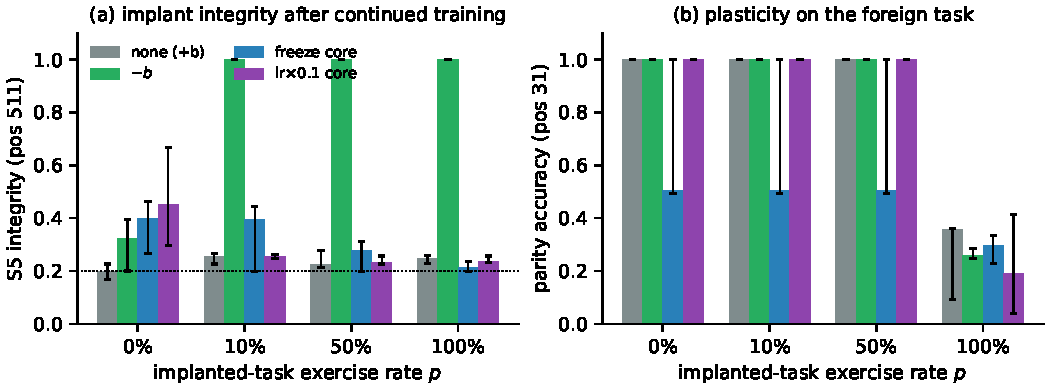
\includegraphics[width=\linewidth]{figs/fig1_fate.pdf}
\caption{\textbf{(a)} End-of-training implant integrity by exercise rate and protection arm
(bars: seed medians; whiskers: seed range; dotted line: chance). Only $-b$ with $p\ge10\%$
retains. \textbf{(b)} Foreign-task (parity) accuracy: freezing the core collapses plasticity;
every other arm learns the foreign task fully at $p<100\%$.}
\label{fig:fate}
\end{figure}

\subsection{The resurrection: concealed, not erased}\label{sec:resurrection}
Why does the exercised (+$b$) implant die even while its task is half the training data? The
companion study's mechanism predicts the answer: it doesn't. We reran the four decisive
conditions ($\{$none, freeze-core$\}\times p\in\{0,100\%\}$, three seeds each; identical
configurations; disclosed as post-hoc exploratory) and evaluated end-of-training integrity twice
--- as trained, and with the additive projection zeroed at inference
(Fig.~\ref{fig:resurrection}):

\begin{itemize}
\item $p{=}100\%$, both arms, all six cells: integrity
$\imRevPhundredNoneBefore$/$\imRevPhundredFreezeBefore$ as trained $\to$ \textbf{exactly
$\imRevPhundredNoneAfter$} with $W_b$ zeroed. The implanted automaton survived $60$ epochs of
training \emph{intact}; cross-entropy grew a bypass around it ($\|W_b e\|\approx
\imRevPhundredNoneBnorm$--$\imRevPhundredFreezeBnorm$) that conceals it behaviorally.
\item $p{=}0\%$, freeze-core, all three cells: $\to\imRevPzeroFreezeAfter$. With the transition
circuit frozen, even training that never exercises the skill leaves it fully recoverable.
\item $p{=}0\%$, unprotected, all three cells: NOT recoverable at depth
($\imRevPzeroNoneAfter$) although in-domain behavior restores ($\imRevPzeroNoneInDom$): with
every parameter free and no exercise, the deep automaton structure genuinely erodes.
\item The bypass norm scales with exercise ($\|W_b e\|$: $\imRevPhundredNoneBnorm$ at $p{=}100\%$
vs.\ $\imRevPzeroNoneBnorm$ at $p{=}0$): loss pressure on the implanted task \emph{feeds} the
parasite, exactly the norm-inflation channel of \citet{howe2026automaton}.
\end{itemize}

The fate taxonomy: an implanted skill under continued training ends \textbf{protected} ($-b$ +
exercise: never harmed), \textbf{concealed} (+$b$ + exercise, or frozen core: behaviorally dead,
fully recoverable by a one-line intervention), or \textbf{eroded} (unprotected \emph{and}
unexercised: deep structure lost). Two consequences. For deliberate skill installation, the
recoverability question --- not the raw-retention question --- is the right one, and the additive
path is the master switch. For the edit-durability literature, which reports decay without a
ground-truth circuit \citep{cheng2025erase,wen2025retention}, our result is a caution: what is
measured as an erased edit may be a concealed one, and the difference matters both for safety
(concealed capabilities can be restored) and for method design (protect the bypass, not the
weights).

\begin{figure}[t]
\centering
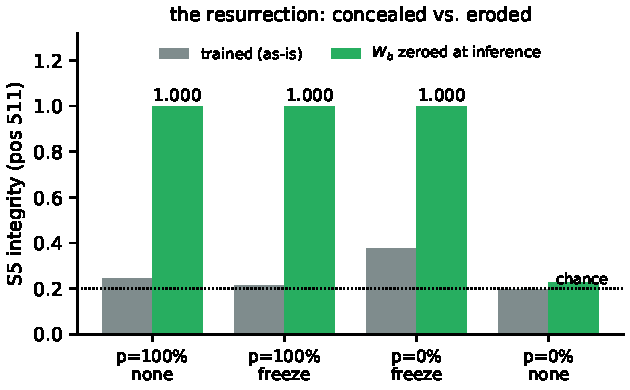
\includegraphics[width=0.62\linewidth]{figs/fig2_resurrection.pdf}
\caption{The b-zero reveal on ``dead'' implants (means over three seeds; post-hoc exploratory):
zeroing the additive projection at inference restores exercised implants and frozen-core implants
to exactly $1.000$; only the unprotected-and-unexercised condition is genuinely eroded.}
\label{fig:resurrection}
\end{figure}

\section{Tier 2: at LM scale, insertion is the bottleneck}\label{sec:tier2}
The pre-registered LM tier (a 30M-parameter DeltaNet-class TinyStories LM from
\citealt{howe2026hygiene}) was designed to measure \emph{retention}: create a toggle-tracking
skill by fine-tuning on a $50\%$ tracking mixture, then watch it decay under pure-LM training with
four protection arms. It never got there --- the frozen creation gate (toggle-8 $\ge0.90$ after
$2{,}500$ steps, one disclosed escalation to $5{,}000$) \textbf{failed}: the pretrained model sat
at exactly chance ($\imLmCreateToggle$, the constant-answer signature) through the full escalation
while mixture loss fell normally.

Two post-hoc controls (labeled) sharpen this into a finding (Fig.~\ref{fig:lm}). A \textbf{cold
control} --- the identical harness, data, optimizer, and batch geometry from \emph{random}
initialization --- acquires the skill by step $\imColdEmergeStep$ and holds it (one $n{=}50$
evaluation flicker aside, visible in Fig.~\ref{fig:lm}). A \textbf{warm
extension} --- the failed checkpoint continued another $10{,}000$ steps
($\imWarmTotalStepsK$k total, $\approx\imBudgetRatio\times$ the cold emergence time) --- stays at
chance at all $21$ evaluations. And the loss ordering is inverted throughout: the pretrained model
has strictly better language quality and lower mixture loss at every step and never acquires the
skill; the random init pays perplexity ($\imColdEndPpl$ vs.\ $\imLmPrePpl$ at the pretrained
start) and gets it almost immediately. The skill is not on the loss-descent path from the
pretrained basin: the pretrained model can answer the tracking checks with a constant policy and
spend its gradient budget polishing everything else, and $300$M tokens of pretraining made that
basin inescapable at this budget --- \emph{warm-start skill-acquisition resistance}, blocked not
delayed, qualitative rather than the quantitative slowdowns of the plasticity literature
\citep{ash2020warm,dohare2024plasticity}.

The program consequence inverts the study's premise: at LM scale via fine-tuning, the bottleneck
for deliberate skill installation is \textbf{insertion}, not retention. That elevates Tier 1's
instrument --- direct weight-space implantation, where insertion is exact by construction and the
protection law governs what happens next --- from toy convenience to the load-bearing route, and
makes ``construct the exact implant inside a real LM layer'' the natural next-scale problem.

\begin{figure}[t]
\centering
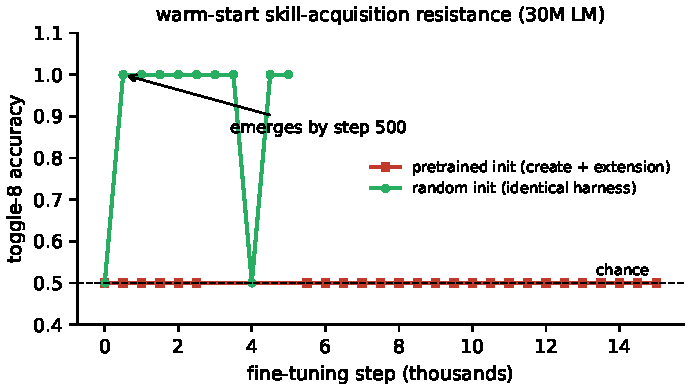
\includegraphics[width=0.66\linewidth]{figs/fig3_lm.pdf}
\caption{Warm-start skill-acquisition resistance (30M LM, identical fine-tuning harness): a
random init acquires toggle tracking by step $\imColdEmergeStep$; the TinyStories-pretrained model
stays at chance through $\imWarmTotalStepsK$k steps at lower loss throughout.}
\label{fig:lm}
\end{figure}

\section{Tier 3: constructing the fate map at LM scale}\label{sec:tier3}
Since fine-tuning cannot insert the skill (Tier 2), we take the route Tier 1 makes available:
\emph{construct} it directly into the trained LM, then continue training and measure its fate. This
is pre-registered separately (freeze before the continued-training battery).

\textbf{The construction obstacle.} A trained tied-embedding LM has no spare residual capacity: over
TinyStories, the least-active residual dimension has standard deviation $\imLmwResidMin$ against a
median of $\imLmwResidMedian$. Donating one attention head is cheap but head-specific
(Fig.~\ref{fig:lm3construct}a: block-$0$ head~$1$ costs $\imLmwHeadOne\%$ perplexity, head~$6$ a
catastrophic $\imLmwHeadSix\%$), and routing the circuit's answer to the logits \emph{in place}
collides with the block's output RMSNorm and drives perplexity to $\approx10^{\imLmwWallLogTen}$.
\textbf{The widened substrate.} Adding one inert $64$-dimensional head (zero-padding every weight)
is verified identity ($\imLmwWidenInertPct\%$ perplexity); implanting the toggle circuit into that
fresh head is then clean, because the new dimensions are exactly zero for real tokens
(Fig.~\ref{fig:lm3construct}b): behavioral toggle $1.00$ through depth $\imLmwWidenDepth$ at
$\imLmwWidenImplantPct\%$ perplexity. An exact skill lives in a real LM and it reads out, free.

\textbf{The battery.} We continue training the implanted widened model for $\imLmwSteps$ steps under
a pre-registered grid: arm $\in\{$all-trainable, freeze-implant$\}$ $\times$ exercise
$p\in\{0,10,50\%\}$, logging behavioral toggle (logits), internal toggle (the implanted head read
directly), and perplexity; after training we re-pin the readout interface and re-measure (the
resurrection probe). Table~\ref{tab:lm3} and Figs.~\ref{fig:lm3traj}--\ref{fig:lm3tax} give the
result, and the Tier-1 taxonomy reproduces:

\begin{table}[t]
\centering\small
\begin{tabular}{llccccc}
\toprule
arm & $p$ & beh.\ start & beh.\ end & internal end & resurrection & ppl end \\
\midrule
\imLmwBatteryRows
\bottomrule
\end{tabular}
\caption{Tier-3 continued-training battery (widened LM, seed 0, $\imLmwSteps$ steps; toggle chance
$0.5$). ``Internal'' reads the implanted head's own computation; ``resurrection'' is behavioral
toggle after re-pinning the readout interface.}
\label{tab:lm3}
\end{table}

\begin{itemize}
\item \textbf{Concealment forms under training and recovers.} All-trainable, $0\%$ exercise:
behavioral toggle decays to chance ($\imLmwBehNoneZeroEnd$) while the internal circuit ends exact
($\imLmwIntNoneZeroEnd$) and re-pinning the readout restores it ($\imLmwResurrectNoneZero$). The
computation survives $\imLmwSteps$ steps of pure-LM training; only its behavioral \emph{expression}
is lost.
\item \textbf{The mechanism is interface drift.} The dedicated tokens' embeddings and the readout
are tied into the shared embedding and take gradients every step, so continued training drifts the
\emph{interface} while the head's computation persists. A $10\%$ exercise trickle pins the interface
(behavior stays $1.00$); freezing the circuit's weights but not its interface is
\emph{counterproductive} (all-trainable co-adapts and re-forms, internal $\imLmwIntNoneZeroEnd$;
freeze/$0\%$ cannot and genuinely erodes, internal $\imLmwIntFreezeZeroEnd$, unrecoverable
$\imLmwResurrectFreezeZero$).
\item \textbf{Skill diffusion.} At $50\%$ exercise behavioral toggle stays $1.00$ while the
single-head internal read drops ($\imLmwIntNoneFiftyEnd$): heavy practice spreads the skill into
redundant routes beyond the implanted head.
\end{itemize}

The concealed/eroded distinction again separates on the internal read (Fig.~\ref{fig:lm3tax}) ---
which, relative to unlearning-robustness detectors \citep{deeb2024weights,lee2026uds}, we can here
\emph{ground} against a known-intact construction rather than infer.

\begin{figure}[t]
\centering
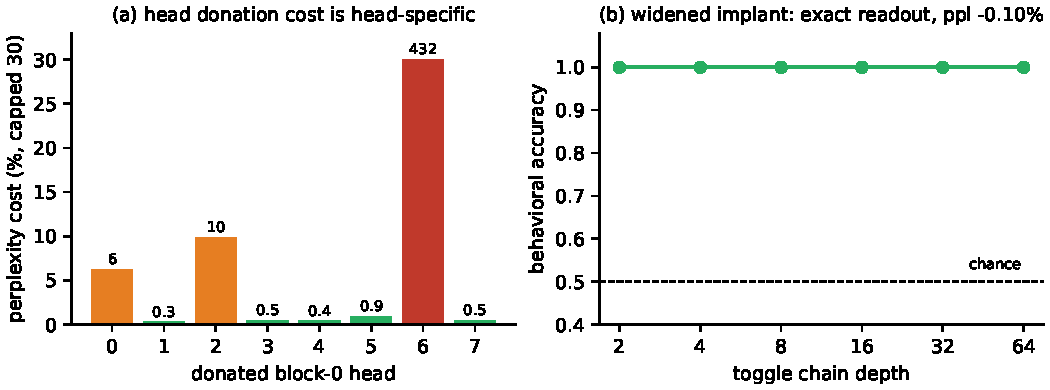
\includegraphics[width=\linewidth]{figs/fig4_lm_construct.pdf}
\caption{\textbf{(a)} Perplexity cost of donating each block-$0$ head (capped $30\%$; head~$6$ is
$\imLmwHeadSix\%$). \textbf{(b)} In the widened substrate the implanted circuit reads out at $1.00$
through depth $\imLmwWidenDepth$, at $\imLmwWidenImplantPct\%$ perplexity.}
\label{fig:lm3construct}
\end{figure}

\begin{figure}[t]
\centering
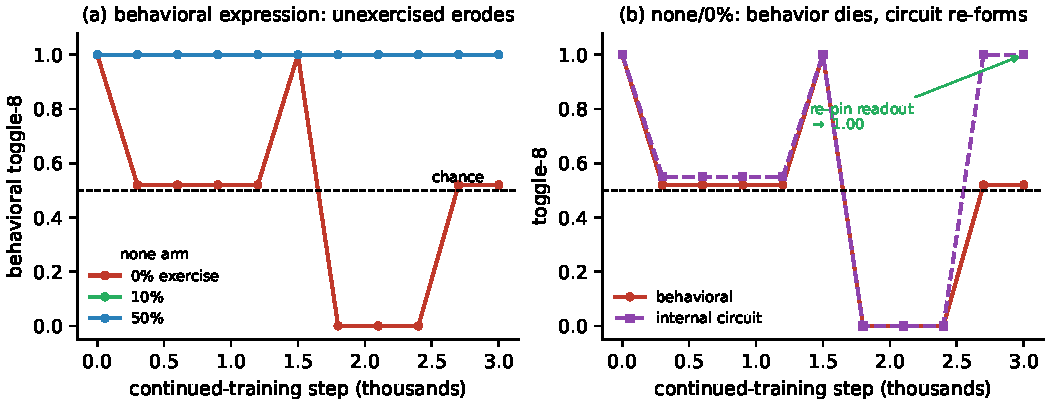
\includegraphics[width=\linewidth]{figs/fig5_lm_traj.pdf}
\caption{\textbf{(a)} Behavioral toggle over continued training (all-trainable arm): unexercised
erodes to chance; a $10$--$50\%$ trickle holds it. \textbf{(b)} all-trainable/$0\%$: behavioral
expression collapses while the internal circuit --- perturbed during training, exact at the end ---
persists; re-pinning the readout restores behavior.}
\label{fig:lm3traj}
\end{figure}

\begin{figure}[t]
\centering
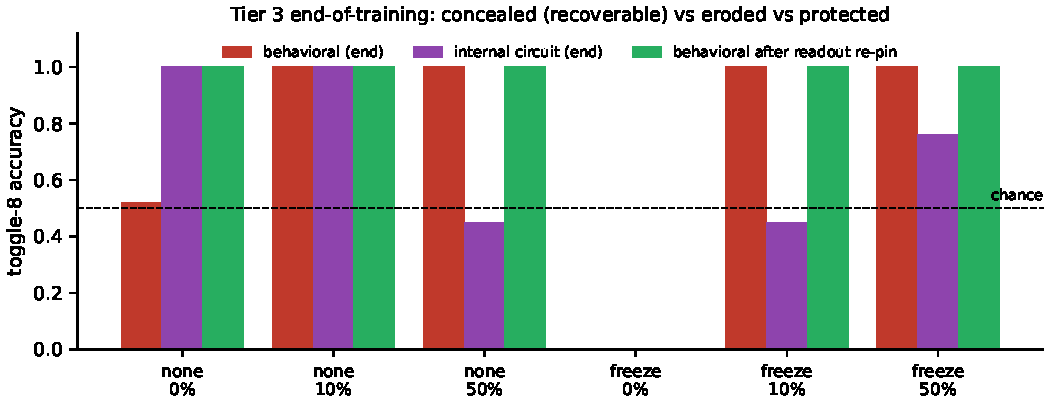
\includegraphics[width=\linewidth]{figs/fig6_lm_taxonomy.pdf}
\caption{Tier-3 end-of-training state per cell: concealed-but-recoverable (all-trainable/$0\%$),
eroded (freeze/$0\%$), and protected (exercised) separate on the internal read, exactly as at toy
scale (\S\ref{sec:resurrection}).}
\label{fig:lm3tax}
\end{figure}

\section{Limitations and disclosures}
Tier 1 is toy-scale by design --- that is what buys the exact ground truth --- with one implant
task ($S_5$), one foreign task (parity on a shared head), one optimizer, and $112$ dimensions; the
protection law and taxonomy are three-seed toy results whose LM-scale analogues are untested
(P4 of \citealt{howe2026hygiene} suggests the LM regime can differ). Three of four frozen Tier-1
predictions failed as frozen; everything in \S\ref{sec:law}--\S\ref{sec:resurrection} beyond IP4
is post-hoc structure requiring pre-registered replication to harden. The reveal reruns duplicate
the original cells' configurations rather than reusing saved weights (checkpoints were not
retained; CUDA nondeterminism makes trajectories near- rather than bit-identical). Tier 2 is one
model, one skill, one fine-tuning recipe, single-seed, with constant learning rate $3\times10^{-4}$
(matched early-phase scale to the from-scratch grid); ``blocked'' is scoped to this budget
($\imWarmTotalStepsK$k steps) and recipe --- curricula, higher learning rates, or partial
re-initialization might break the resistance, and distinguishing those is future work, not a
counter-claim. \textbf{Tier 3} shares Tier 1's toy-skill scope (toggle, one head, one seed) and
adds its own: the widened substrate \emph{adds} capacity rather than implanting into the model
as-is (the in-place readout is blocked by the dense-stream RMSNorm, itself reported); the
continued-training setup drifts perplexity $+\imLmwDriftFloorPct\%$ even at zero exercise (learning
rate not tuned for minimal-drift continuation), so absolute perplexity is not a clean cost
measurement, though the toggle-integrity findings are within-run relative. \textbf{On the
unlearning connection}: Tier 3 is a mechanistic case study on a \emph{constructed} skill under
generic continued training, not a targeted unlearning method on natural knowledge; that
suppression can spare the weights is established \citep{deeb2024weights,lee2026uds,xu2026reversibility},
and we neither claim that as new nor propose a detector --- our added value is the ground-truth
handle and the interface-drift mechanism, and the recovery here is white-box, not an adversary
acting on a released checkpoint.

\section{Reproducibility}
The full record --- pre-registrations (frozen before any run), all Tier-1 cell artifacts, reveal
and control artifacts, LM logs, the Tier-3 construction scripts and $6$-cell battery, verdicts, and
this paper's regeneration pipeline --- is published in the \texttt{implant/} and \texttt{lmimplant/}
directories of \url{https://github.com/gunnerhowe/automaton-underneath} (companion records:
\texttt{statetrack\_note/}, \texttt{twogap/}, \texttt{prodgate/}). Key commits (private working
repository; access on request): Tier-1/2 pre-registration freeze \texttt{39b2b88}, Tier-1 verdicts
\texttt{7d0d8d8}, Tier-2 verdicts \texttt{0786a3e}; Tier-3 construction \texttt{1fd5cf4} and
battery pre-registration/verdicts. Every number here is a macro generated by
\texttt{gen\_numbers.py} from committed artifacts (Tier-3 numbers read the \texttt{lmimplant/}
\texttt{facts.json} and battery cells) and byte-verified by \texttt{verify\_regen.py}. Total
compute: $\approx5$ GPU-hours (Tier 1 $+$ reveal), $\approx7$ (Tier 2), $\approx2.5$ (Tier 3) on
one RTX 3080.

\bibliographystyle{plainnat}
\bibliography{references}

\end{document}
